%!TEX program = xelatex
%!BIB program = bibtex

\documentclass[en,black,12pt,normal]{elegantnote}
\usepackage{float}
\usepackage{subfigure}


\newcommand{\upcite}[1]{\textsuperscript{\textsuperscript{\cite{#1}}}}

\title{Practical 7 Homology modeling}
\author{WenYuan Jiang\\ID: 1951510}
\institute{School of Life Science, Tongji University}
%\version{1.00}
\date{\today}
\lstset{basicstyle=\footnotesize\ttfamily}
\AtBeginEnvironment{lstlisting}{\linespread{0.75}\selectfont}

\begin{document}

\maketitle

\section{Homology modeling}

\subsection{Please briefly introduce at least 3 protein 3D structure prediction tools, including pros and cons.}

\begin{enumerate}
    \item SWISS-MODEL\upcite{guex1997swiss}
    \begin{itemize}
        \item PRO: Accurate if homology exists. Costs little computation, thus being fast.
        \item CON: Previous datasets are needed. May fail if no homology found.
    \end{itemize}
    \item I-TASSER\upcite{zhang2008tasser}
    \begin{itemize}
        \item PRO: Produces relative accurate results even no similar sequences exists.
        \item CON: Previous datasets are also needed. Takes longer time and is less accurate.
    \end{itemize}
    \item ROSETTA\upcite{rohl2004protein}
    \begin{itemize}
        \item PRO: No previous dataset is needed, that is \textbf{ab initio}. Can be used for completely unknown proteins.
        \item CON: Much computational resources is needed, thus being extremely slow. Results is not accurate compared with the other tools.
    \end{itemize}
\end{enumerate}


\subsection{Please perform homology modeling to get the predicted 3D structure of your protein sequence.}

The protein sequence used in homology modeling is shown below:

\begin{lstlisting}
PISSKPVIVTGLQDTTVSSDSVAKFAVKATGEPRPTAIWTKDGKA
ITQGGKYKLSEDKGGFFLEIHKTDTSDSGLYTCTVKNSAGSVSSS
CKLTIKAI
\end{lstlisting}

This sequence is a subunit of the \textbf{Human Titin}. (PDB 3PUC) And its original structure is shown below.


\begin{figure}[H]
    \centering
    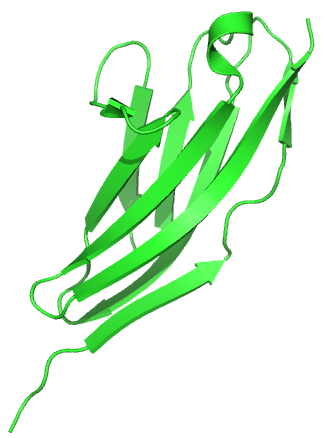
\includegraphics[width=0.3\textwidth]{1}
    \caption{Sturcture of 3PUC}
    \label{3PUCG}
\end{figure}

As can be seen on the figure above, the 3PUC has several anti-parallel beta-sheets and a small aplha-helix, linked by random peptide chains.


The tool used is \textbf{SWISS-MODEL}, and the results is shown in the figures below.

\begin{figure}[H]
    \centering
    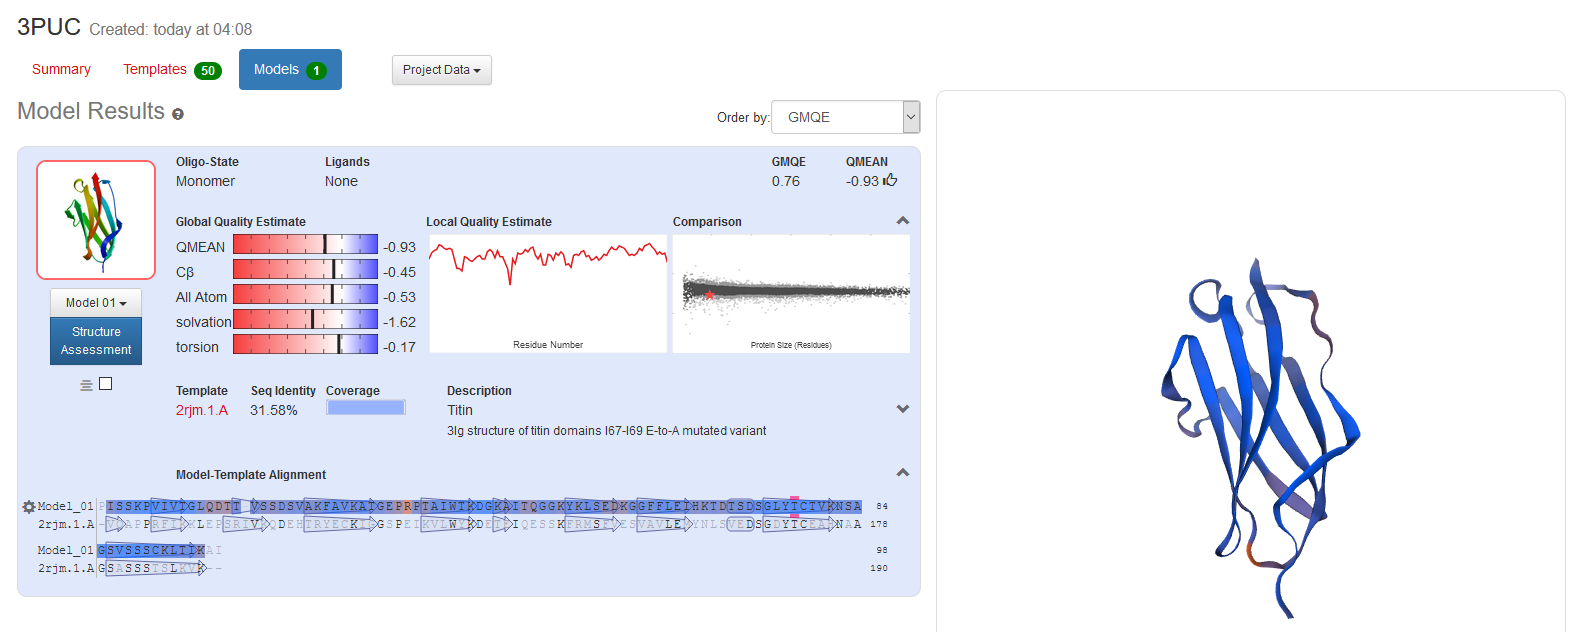
\includegraphics[width=1\textwidth]{5}
    \caption{Summary of \textbf{SWISS-MODEL} results (zoom in for more details)}
    \label{SMRES}
\end{figure}

\section{Optional exercise}


\subsection{Visualize structure files from the Protein Data Bank (PDB)}

The author prefers to use CLI (command-line interface) to operate PyMOL, for its unambiguity and effeciency.
How to use GUI to perform visualization can be found in the Supplementary materials.

Open PyMOL shell, and execute the following command:

\begin{lstlisting}
fetch 3PUC
remove solvent
remove inorganic
set two_sided_lighting,1
set cartoon_fancy_helices, 1
set cartoon_fancy_sheets, 1
spectrum
ray 
png 1.png
\end{lstlisting}

The generated figure is shown below.

\begin{figure}[H]
    \centering
    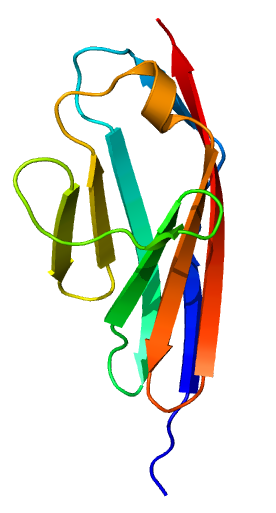
\includegraphics[width=0.3\textwidth]{2}
    \caption{PyMOL Generated Figure}
    \label{3PUCCOL}
\end{figure}


\subsection{Comparing models with experimental structures}
Open the target pdb using PyMOL or any other tool (such as RasMol or MOE). 
Load template pdb and compare it. Notice how similar they are.


Download the pdb file from SWISS-MODEL and then open PyMOL shell. 
Execute the following command:

\begin{lstlisting}
fetch 3PUC
remove solvent
remove inorganic
set two_sided_lighting,1
set cartoon_fancy_helices, 1
set cartoon_fancy_sheets, 1
color marine, 3puc
load model_01.pdb
align model_01, 3puc 
color red model_01
ray 
png 2.png
\end{lstlisting}

The generated figure is shown below.

\begin{figure}[H]
    \centering
    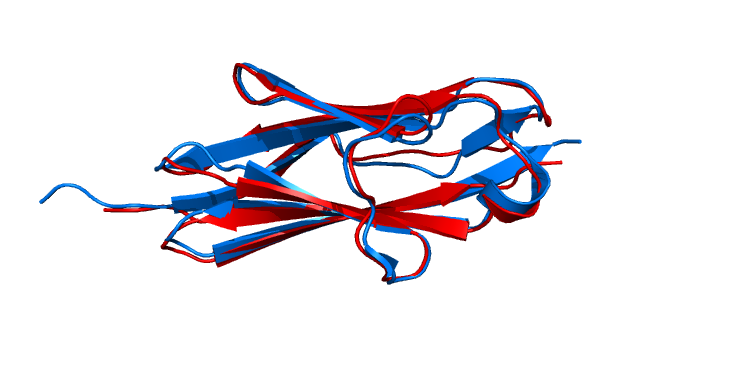
\includegraphics[width=0.9\textwidth]{r1}
    \caption{PyMOL Generated Figure}
    \label{3PUCALI}
\end{figure}


The logs generated by PyMOL is listed below:

\begin{lstlisting}
PyMOL>align model_01, 3puc
 Match: read scoring matrix.
 Match: assigning 95 x 99 pairwise scores.
 MatchAlign: aligning residues (95 vs 99)...
 MatchAlign: score 484.000
 ExecutiveAlign: 690 atoms aligned.
 ExecutiveRMS: 41 atoms rejected during cycle 1 (RMSD=1.60).
 ExecutiveRMS: 38 atoms rejected during cycle 2 (RMSD=1.20).
 ExecutiveRMS: 29 atoms rejected during cycle 3 (RMSD=1.03).
 ExecutiveRMS: 15 atoms rejected during cycle 4 (RMSD=0.93).
 ExecutiveRMS: 13 atoms rejected during cycle 5 (RMSD=0.89).
 Executive: RMSD =    0.854 (554 to 554 atoms)
\end{lstlisting}


\textbf{What is the root-mean-squared (RMS) deviation between the structures?}
According to the log produced by the program:
\begin{lstlisting}
 Executive: RMSD =    0.854 (554 to 554 atoms)
\end{lstlisting}
RMS of the structures is 0.854 Å, which is a good-enough modeling from the sequence.

\textbf{How many atoms were used for the calculation of the RMS values?}
According to the log produced by the program:
\begin{lstlisting}
 Executive: RMSD =    0.854 (554 to 554 atoms)
\end{lstlisting}
554 atoms were used for the calculation of the RMS values.


\section{Discussion}

Using Homology modeling for a small peptide chain, like the one on the report, 
can give out reasonable outputs if similar sequences can be found in the datasets.

For larger unknown sequences, although the author did not test some larger proteins,
from the results of other fellows, the overall accuracy is still acceptable, but in
some linking regions, error can be big.

CLI can be useful for batch processing of visualization tasks, with scripts written for automated
modeling or dicking.


\section{Supplementary materials: Tutorials and Notes}

\subsection{Visualize structure files from the Protein Data Bank (PDB)}

Before you begin on your 3D structural analysis, you will first have to obtain the 3D structure(s) of interest. 
There are two ways of retrieving 3D structure files – through online 3D structure databases or structural modeling (or prediction) software. 
Since the 3D structure of SARS-coV-2 has been determined and is available online, we will retrieve the relevant structure file from the Protein Data Bank (PDB).

\begin{itemize}
    \item Prepare your pdb file. 
    \item Open Phymol, go to “File” and then select “Open...”. open your pdb.
\end{itemize}


\subsubsection{Display the structure using the “cartoons” representation}
At the main window, beside the selection 1RUZ, click “S” (Show) -> cartoon. 
You will see that the cartoon display will be loaded over the original “sticks” display. Paste the screen. 
You can change the display to cartoon only by clicking “S” (Show) -> as- > cartoon.


\subsubsection{Next, color the structure with one single color.}
At the main window, beside the selection your pdb, 
click “C” (Color) and select your favorite color from the list and paste the screen.


\subsubsection{Now, you will use the mouse buttons to visualize the structure.}
Clicking and dragging the mouse buttons (left, middle and right) and/or pressing with other keys (Ctrl, Shift) manipulates the structure. 
Some of the regularly used features are described below:

Viewing the structure

\begin{itemize}
    \item To rotate the structure, left-click the mouse button and drag the mouse.
    \item To zoom in and out, right-click the mouse button and drag the mouse up/down. To move the structure, click and drag the middle mouse button.
    \item To reset the structure back to its original position, click on the “Reset” button at the external GUI window.
\end{itemize}



\subsection{Comparing models with experimental structures}
Open the target pdb using PyMOL or any other tool (such as RasMol or MOE). 
Load template pdb and compare it. Notice how similar they are.

\subsubsection{For a more quantitative comparison, you can align and superimpose both structures in PyMOL. }
To do that, make sure you have loaded both structures into the same window. 
At the PyMOL main window, select a structure, then click the Action (A) button -> Align -> To Molecule and select name of the structure you want to align to.



\subsubsection{Inspect the output of the structural alignment at the PyMOL external GUI window.}



You should see a few lines describing the alignment process.

\textbf{What is the root-mean-squared (RMS) deviation between the structures?}


\textbf{How many atoms were used for the calculation of the RMS values?}

Note: The structural match between the two molecules is measured by root-mean-squared deviation (RMS deviation or RMSD) of the aligned atoms. In structural biology, RMSD are typically measured in Ångström (Å). The larger the RMSD value, the larger the difference between the template and the super-imposed structure. A RMSD value of less than 1.5Å is usually considered to be significant.

The “align” command in PyMOL automatically generates a sequence alignment to select the right atoms to compare and yields the minimal RMS deviation (or RMSD) between the aligned structures.

By rotating the molecule around, you will notice that this molecule is composed of three polypeptide subunits that are almost copies of each other forming a trimer.

Selecting parts of the structure

To select any atom of the structure, you will have to first change the select mode to “Atoms”. You can do this by clicking on the text beside the field “Selecting” multiple times.

Now, clicking on any part of the 3D structure will identify the atom in the external GUI window. Try clicking on any part of the 3D structure and then check the name of the atom in the external GUI window.

Notice that every time u click on an atom, a new selection (sele) will appear at the main window. If you click on more than 1 atom, all the atoms will be grouped under the same selection.

Each selection can be manipulated individually using the GUI menu buttons (S (show), C (color) etc). For example, you can change the color of the selected atom, or the whole residue which the atom belongs to by clicking on the C button corresponding to the selection.




\bibstyle{unsrt}
\bibliography{references}{}
\end{document}
